\documentclass[aspectratio=34]{beamer}

% Remove the gratuituous footer
\setbeamertemplate{footline}{}
\setbeamertemplate{navigation symbols}{}
%\renewcommand{\insertnavigation}[1]{}

%\usepackage{syntonly}
%\syntaxonly

\usepackage{graphicx}

%\usepackage{rotating}
\usepackage{algorithm}
\usepackage{algorithmicx}
\usepackage{algpseudocode}
\usepackage{xcolor}
\usepackage{setspace}
\usepackage{amsmath}
\usepackage{amsthm}
\usepackage{amssymb}

\makeatletter
\renewcommand{\ALG@beginalgorithmic}{\scriptsize}
%%%%%%%%%%%%%%%%%%%%%%%%%%%%%% Textclass specific LaTeX commands.
\usepackage[natbibapa]{apacite}
\theoremstyle{plain}
\makeatother

\usepackage{caption}
\usepackage{subcaption}

\DeclareMathOperator{\conv}{conv}
\DeclareMathOperator{\st}{s.t.}
\DeclareMathOperator{\dom}{dom}
\DeclareMathOperator{\im}{im}
\DeclareMathOperator{\Ne}{Ne}
\DeclareMathOperator{\sign}{sign}
\DeclareMathOperator{\Var}{Var}
\DeclareMathOperator{\diag}{diag}
\DeclareMathOperator{\vvec}{vec}

%\graphicspath{{"Learning Matchings/figs/"},{../fig/}}

%\usepackage{beamerthemesplit}

% Make footnotes visible. Stolen from http://tex.stackexchange.com/questions/5852/beamer-footnote-text-collides-with-navigation-symbols
\addtobeamertemplate{footnote}{\vspace{-6pt}\advance\hsize-0.5cm}{\vspace{6pt}}
\makeatletter
% Alternative A: footnote rule
\renewcommand*{\footnoterule}{\kern -3pt \hrule \@width 2in \kern 8.6pt}
% Alternative B: no footnote rule
% \renewcommand*{\footnoterule}{\kern 6pt}
\makeatother

\usepackage[natbibapa]{apacite}

\title{Expanding Compressed Learning}
\author{Kevin Shi \and Kui Tang}
\institute{Columbia University}

\date{11 Dec. 2015}

\begin{document}

\frame{\titlepage}

% Overall outline
\AtBeginSection[]
{
\begin{frame}<beamer>
\frametitle{Outline}
\tableofcontents[currentsection]
\end{frame}
}

\section{Compressed Learning}

\subsection{Review of Calderblank et. al. 09}

\begin{frame}
\frametitle{Learning Compressively-Sensed Data}
\begin{figure}
    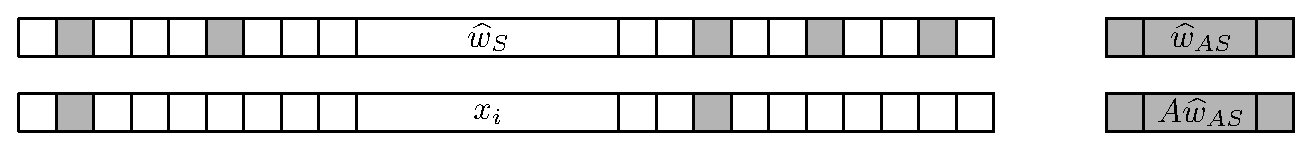
\includegraphics[width=\columnwidth]{S_vs_AS.pdf}
    \caption{\label{fig:S_vs_AS}Sample space $S$ and measurement (compressed) space $AS$.}
\end{figure}
\begin{itemize}
    \item There exist training data ${(x_i,y_i)} \subset \mathbb{R}^n \times {-1,1}$ where the $x_i$ are $k$-sparse, learn binary classifier $f : \mathcal{X} \rightarrow {-1,1}$.
    \item We observe compressively-sensed measurements ${(Ax_i,y_i)} \subset \mathbb{R}^M \times {-1, 1}$ for a $(2k,\epsilon)$ RIP $m \times n$ matrix $A$.
    \item Two options
    \begin{itemize}
        \item Recover $n$-dimensional sparse vectors, learn classifier in the high dimensional space.
        \item \textbf{Learn classifier directly in the compressed space!}
    \end{itemize}
\end{itemize}
\end{frame}

\begin{frame}
\frametitle{Support Vector Machine Review}
\begin{itemize}
    \item We minimize the hinge loss, which on one example is $H(x,y;w) = \max{0, 1 - yw^\top x}$
    \item The true hinge loss on distribution $\cal D$ is $H_{\cal D}(w) = E_{(x_i,y_i) \sim {\cal D}} [1 - y_i w^\top x_i]$
    \item The true regularization loss is $L(w) = H_{\cal D}(w) + \frac{1}{2C}\left\Vert w \right\Vert$.
    \item The trained SVM classifier $\widehat{w}_S$ can be written as $$\widehat{w}_S = \sum_i \alpha_i y_i x_i $$ where $0 \leq \alpha_i \leq C/M$ and $\left\Vert \widehat{w}_S \right\Vert \leq C$.
    \item If $w^*$ is the best SVM classifier over $\cal D$, then with probability $1 - \delta$, we have \citep{Sridharan08} $$L_{\cal D}(\widehat{w}_S) \leq L_{\cal D}(w^*) + O\left(C \log \frac{1}{\delta} / M\right)$$
\end{itemize}
\end{frame}

\begin{frame}
    \frametitle{Compressed Learning Bound}
    Main result is
    \[
    L_{\cal D}(\widehat{z}_{AS}) \leq L_{\cal D}(w^*) + O(CR^2\epsilon + C\log\frac{1}{\delta} / M)
    \]
    \begin{figure}
        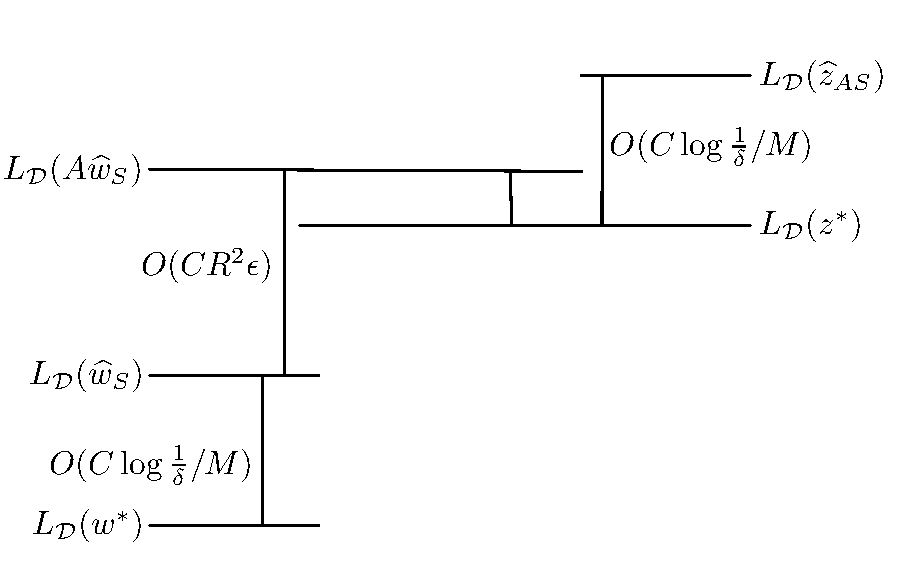
\includegraphics[width=\columnwidth]{bounds_argument_figure.pdf}
    \end{figure}
\end{frame}

\begin{frame}
\frametitle{RIP for Dot Products}
\begin{theorem}[\citet{Calderbank09}]
    \label{theorem:kernel} Let $A_{m\times n}$ be $(2k,\epsilon)$-RIP,
    $x,x'$ two $k$-sparse vectors in $\mathbb{R}^{n}$ with $\left\Vert x\right\Vert ,\left\Vert x\right\Vert \leq R$.
    Then
    \[
        (1+\epsilon)x^{\top}x'-2R^{2}\epsilon\leq\left(Ax\right)^{\top}\left(Ax'\right)\leq(1-\epsilon)x^{\top}x'+2R^{2}\epsilon
    \]
\end{theorem}
\end{frame}

\begin{frame}
\frametitle{Applying Dot-RIP to SVM Loss}
\begin{itemize}
    \item Suppose we train a classifier $\widehat{w}_S$ in the high-dimensional space.
    \item Project to low dimensional space, getting classifier $A\widehat{w}_S$.
    \item A key result is to show that projection does not increase the loss too much:
        \[
            L_{\cal D}(A\widehat{w}_S) \leq L_{\cal D}(\widehat{w}_S) + O(CR^2\epsilon) \label{eq:loss-bound}
    \]
    \item $L$ contains terms of the form $y_iw_i^\top x_i$ and $\Vert w \Vert$.
    \item Use kernel representation $$\widehat{w}_S = \sum_i \alpha_i y_i x_i $$ to write~\eqref{eq:loss-bound} in terms of $(A\widehat{w}_S)^\top (Ax)$ and $\widehat{w}_S^\top x$, and use Theorem~\label{theorem:kernel} to get result.
    \item Technical issues with signs and cases... tedious but it works out.
\end{itemize}
\end{frame}

\begin{frame}
    \frametitle{Putting it Together}
    $$L_{\cal D}(\widehat{z}_{AS}) \leq L_{\cal D}(w^*) + O(CR^2\epsilon + C\log\frac{1}{\delta} / M)  $$
    \begin{figure}
        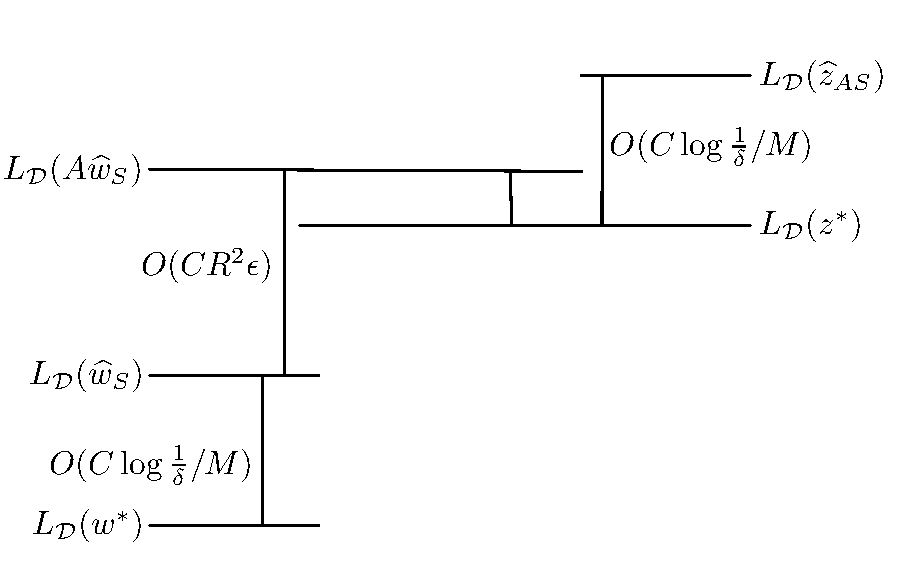
\includegraphics[width=\columnwidth]{bounds_argument_figure.pdf}
    \end{figure}
\end{frame}

\subsection{Extension to Regression}

\begin{frame}
\frametitle{Support Vector Regression}
\begin{itemize}
    \item We have continuous $y$ and use the $\rho$-insensitive \emph{tube loss}
    \[
    T(x,y;w)=\max\left\{ y-w^{\top}x-\rho,w^{\top}x-y-\rho,0\right\} \label{eq:epsilon-insensitive}
    \]
    \item The dual (kernel) representation of the learned classifier is
    \[
    w=\sum_{i}\left(\alpha_{i}-\alpha_{i}^{*}\right)x_{i}\label{eq:dual-w}
    \]
\item (Almost) the same projection bound holds! Need another term in $\rho$:
    \[
    T_{{\cal D}}(A\widehat{w}_{S})\leq T_{{\cal D}}(\widehat{w}_{S})+O(CR^{2}\epsilon + \rho)\label{eq:dist-T-bound}
    \]
\end{itemize}
\end{frame}

\begin{frame}
    \frametitle{Compressed Learning for Support Vector Machines}
    \begin{itemize}
        \item The loss function has 3 cases
        \[
        T(x,y;w)=\begin{cases}
        y-w^{\top}x-\rho & (+)\quad y-w^{\top}x-\rho>0\\
        w^{\top}x-y-\rho & (-)\quad w^{\top}x-y-\rho>0\\
        0 & (0)\quad\left|y-w^{\top}x\right|\leq\rho
        \end{cases}
        \]
        \item The difference $T_{{\cal D}}(A\widehat{w}_{S}) - T_{{\cal D}}(\widehat{w}_{S})$ needs to be evaluated for 9 cases (some trivial).
        \item Supporting lemmas also need to be upgraded to handle negative cases.
    \end{itemize}
\end{frame}

\subsection{Other Attempted Generalizations}

\begin{frame}
    \frametitle{Attempts to Generalize to other Kernels}
    \begin{itemize}
        \item Recall the RIP for linear kernels:
        \[
        (1+\epsilon)x^{\top}x'-2R^{2}\epsilon\leq\left(Ax\right)^{\top}\left(Ax'\right)\leq(1-\epsilon)x^{\top}x'+2R^{2}\epsilon
        \]
        \item The squared exponential kernel has with variance $\sigma^{2}$ and length scale $\ell$ is
        \begin{equation}
        k(x,x')=\sigma^{2}\exp\left(-\frac{\left\Vert x-x'\right\Vert _{2}^{2}}{2\ell^{2}}\right)\label{eq:kSE}
        \end{equation}
        \item We have obtained
        \begin{equation}
        \exp(-2\epsilon R-\epsilon^{2}R)k(x,x')\leq k(Ax,Ax')\leq\exp(2\epsilon R)k(x,x')\label{eq:exp-bound}
        \end{equation}
        \item Both the $(1\pm\epsilon)$ and $2R^2\epsilon$ terms are exponentiated.
        \item Tried Matern and rational quadratic kernels... no luck.
    \end{itemize}
\end{frame}

\begin{frame}
    \frametitle{Attempts to Generalize to Linear Regression}
    \begin{itemize}
        \item Classical analysis: suppose $Y = X\beta + \epsilon$ where $\epsilon_i \sim \mathcal{N}(0, \sigma^2)$.
        \item $Y$ random, $X$ and $\beta$ fixed.
        \item The measure of generalization error is \emph{risk}, e.g. expected squared error under the true distribution:
        \begin{eqnarray*}
        E_{Y}\left[\frac{1}{n}\left\Vert Y-X\widehat{\beta}\right\Vert ^{2}\right] & = & E_{Y}\left[\left\Vert \widehat{\beta}-\beta\right\Vert _{\Sigma}^{2}\right]\\
         & = & E_{Y}\left[\left\Vert \widehat{\beta}-\overline{\beta}\right\Vert _{\Sigma}^{2}\right] + E_{Y}\left[\left\Vert \overline{\beta}-\widehat{\beta}\right\Vert _{\Sigma}^{2}\right]
        \end{eqnarray*}
        where $\Sigma = \frac{1}{n} X^\top X$ and $\widehat{\beta} = E_Y[\widehat{\beta}]$ and $\left\Vert x \right\Vert_C = x^\top C x$.
        \item For both linear and ridge ($\ell_2$ regularized) regression, $\widehat{\beta} = \widehat{\beta}(X, Y, \lambda)$  available in closed form.
    \end{itemize}
\end{frame}

\begin{frame}
\frametitle{Problem with Linear Regression}
\begin{itemize}
    \item Again, let's compute the risk of the projected model $A\widehat{\beta}_{AS}$.
    \item The \emph{variance} of the this estimator is
\[
E\left[\left\Vert A\widehat{\beta}_{S}-A\overline{\beta}_{S}\right\Vert _{A\Sigma A^{\top}}^{2}\right]=E\left[\left\Vert \widehat{\beta}_{S}-\overline{\beta}_{S}\right\Vert _{A^{\top}A\Sigma A^{\top}A}^{2}\right]
\]
    \item The term $E\left[\left\Vert \widehat{\beta}_{S}-\overline{\beta}_{S}\right\Vert _{\Sigma}^{2}\right]$ is the variance of the estimator in the high-dimensional space $\widehat{\beta}_S$.
    \item The norm $\left\Vert x \right\Vert_{A^\top A \Sigma A^\top A}$ contains the factor $A^\top Ax$.
    \item But RIP doesn't apply here because $Ax$ is no longer sparse, and $A^\top$ does not have interesting properties.
    \item \textbf{Or am I missing something here?}
\end{itemize}
\end{frame}

\section{Explicit RIP Constructions}

\subsection{}
\begin{frame}
\frametitle{RIP constructions with $m = \tilde{O}(k)$}

\begin{itemize}
\item Draw a random matrix with entries sampled from $\mathcal{N}(0,1/m)$.

\item Draw a random matrix with entries sampled from $\left\{+\frac{1}{\sqrt{m}}, -\frac{1}{\sqrt{m}}\right\}$ with Bernoulli parameter $0.5$. 
\end{itemize}
\begin{theorem}
	With high probability the random matrix $\Phi$ sampled from either distribution above satisfies 
	
	\[(1-\epsilon)\|x\|_2^2 \le \|\Phi x\|_2^2 \le (1+\epsilon)\|x\|_2^2\]
	
	for all $k$-sparse $x$.
\end{theorem}

\end{frame}

\begin{frame}
\frametitle{But...}
\begin{theorem}[\cite{Bandeira12}]
Given a matrix $\Phi$ and parameters $(k,\epsilon)$, certifying whether $\Phi$ is $(k,\epsilon)$-RIP is NP-hard. 
\end{theorem}
\end{frame}

\begin{frame}

\includegraphics[width=4in]{rip.jpg}
\end{frame}


\subsection{Bipartite graph model of measurement}
\begin{frame}
\frametitle{Bipartite graph model of measurement}	
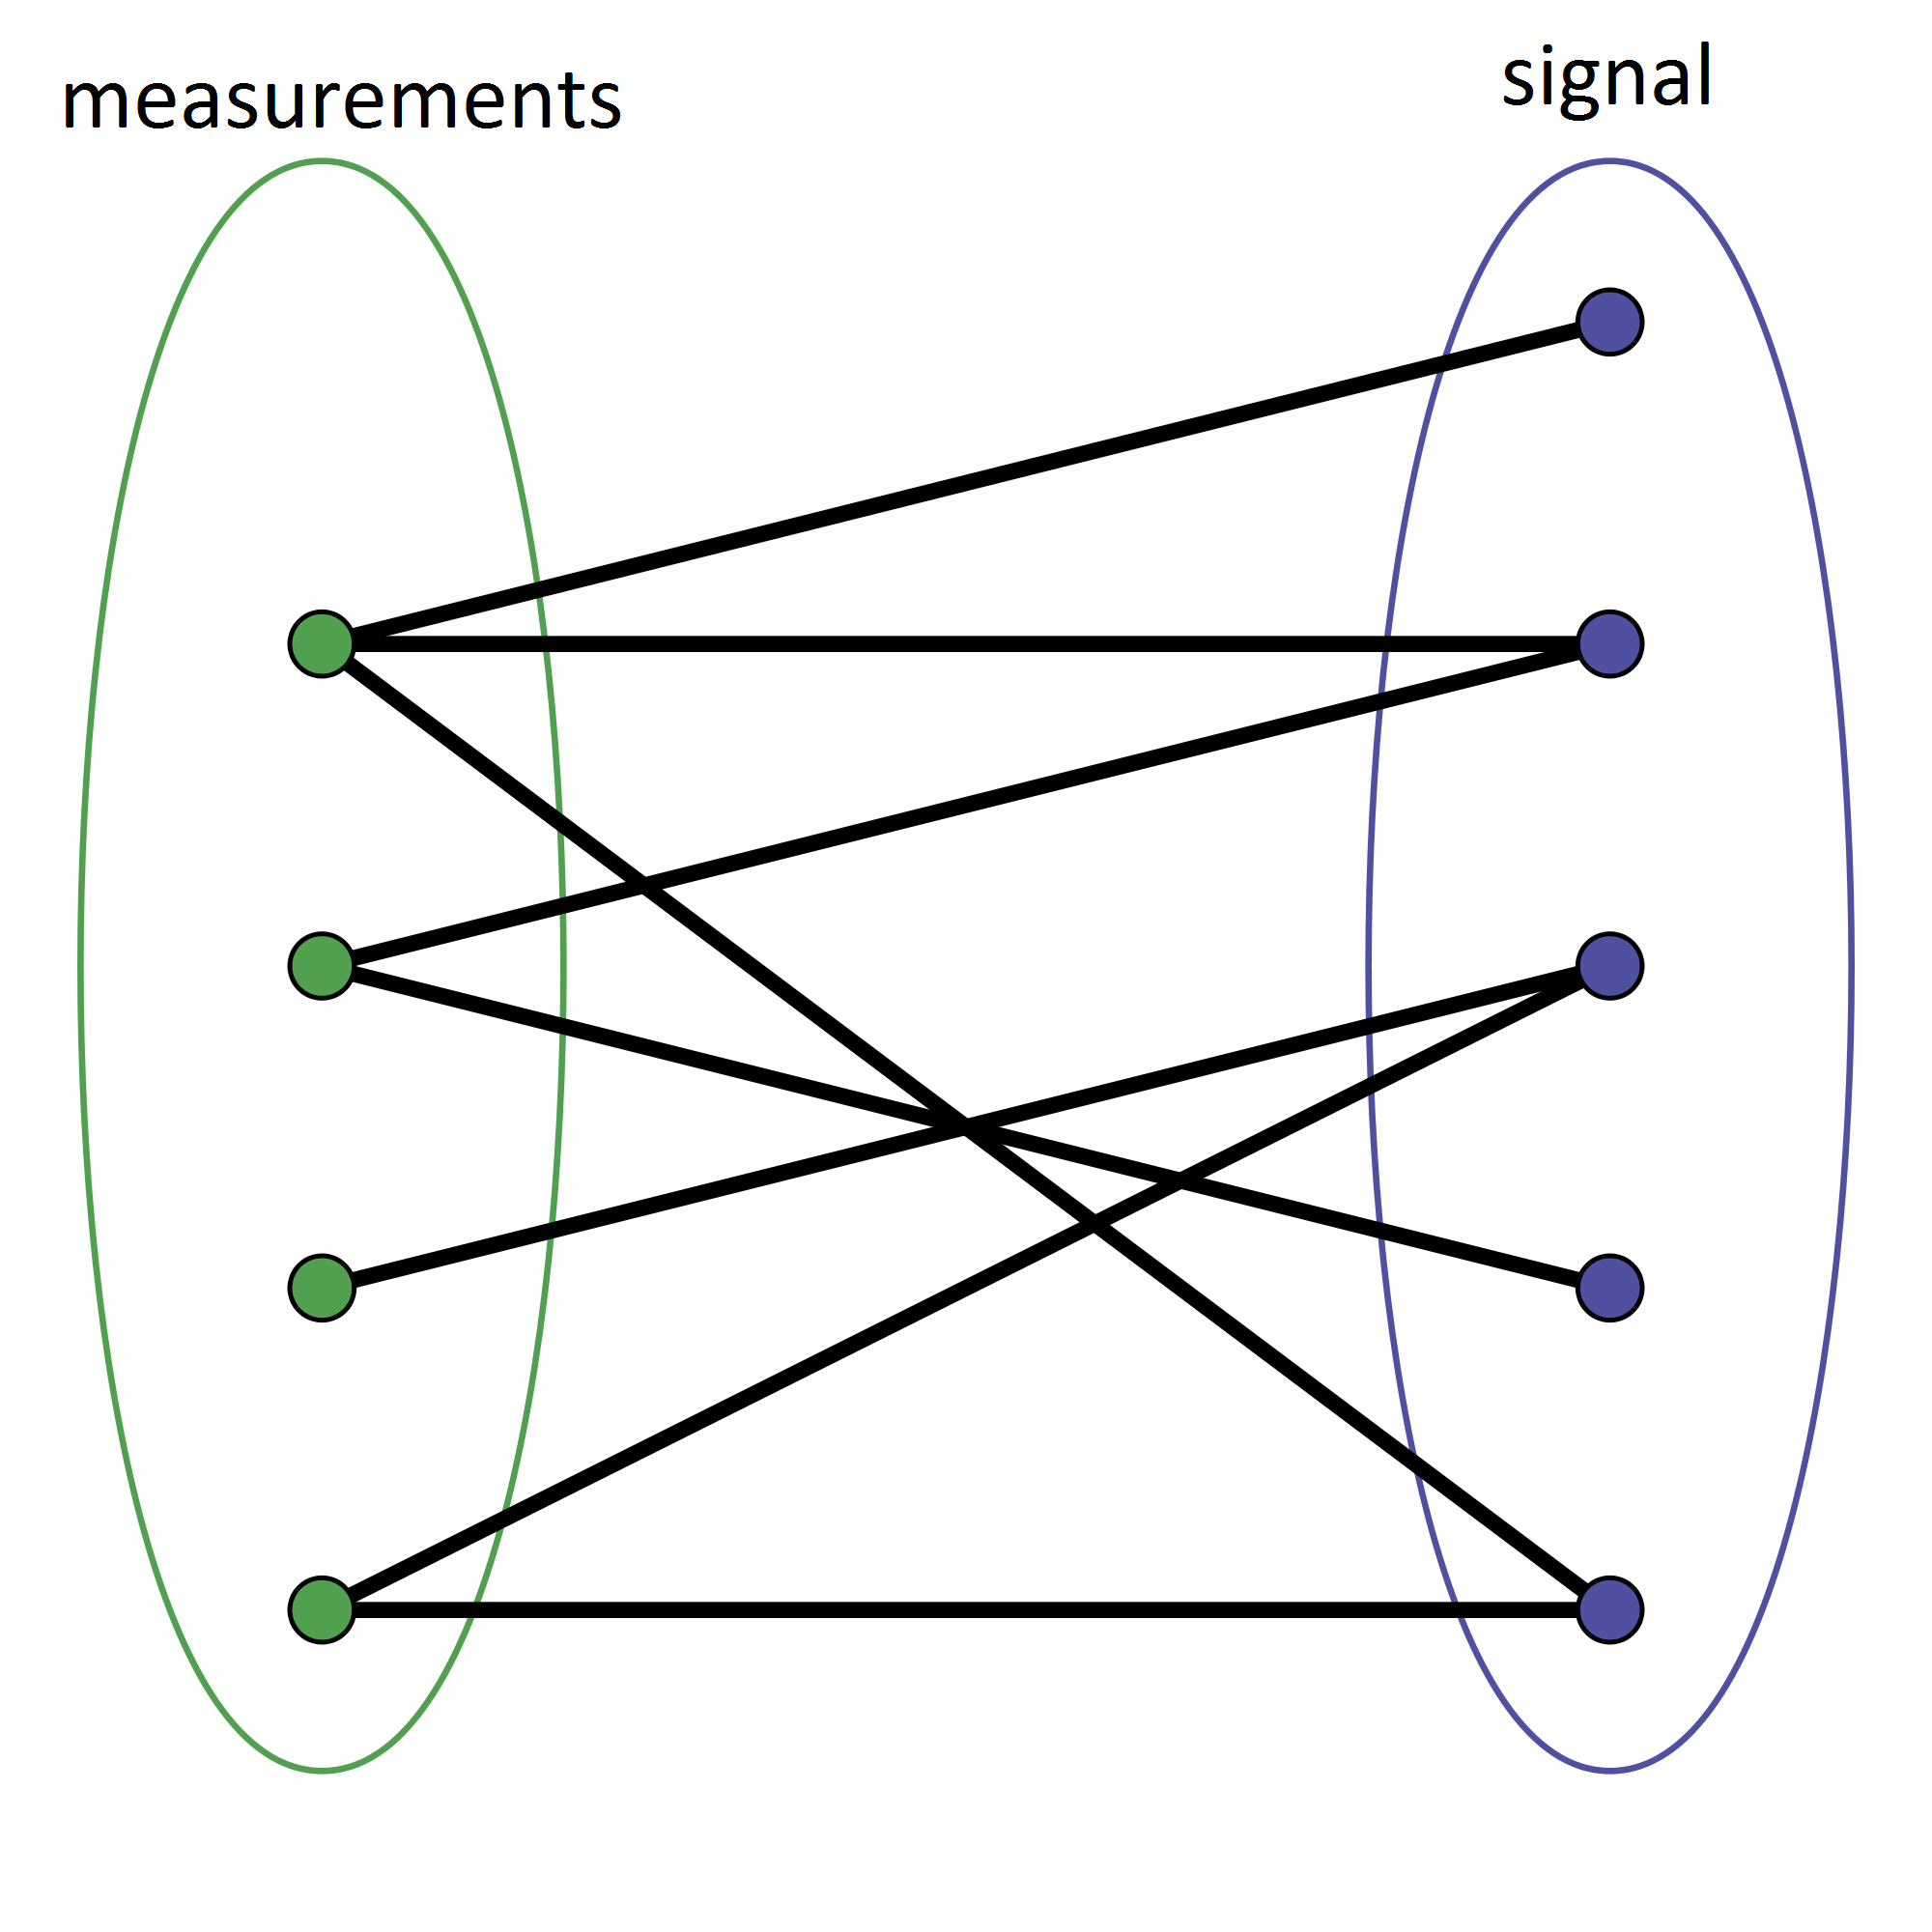
\includegraphics[width=3in]{bpgraph.png}
\end{frame}

\begin{frame}
\frametitle{Expander graphs}
\begin{itemize}
	\item Expander graphs capture many properties of random graphs, but can be constructed deterministically. 
	\item Expander graphs can also be constructed probabilistically, and the graph expansion property can be certified. 
\end{itemize}

\begin{definition}[Vertex expansion]
	Let $G = (A,B,E)$ be a bipartite graph with left degree $d$. G has $(k,\epsilon)$-vertex expansion if for every subset $X \subset A, |X| \le k$, the set of neighbors $N(A) = \{j \in B \, | \, \exists \, i \in X, (i,j) \in E\}$ has size at least $|N(A)| \ge (1-\epsilon)d|X|$.
\end{definition}

\end{frame}

\begin{frame}
    \frametitle{Explicit RIP for $\ell_1$-norm}
    \begin{theorem}[\cite{Berinde2008}]
    Let $(A,B,E)$ be a bipartite expander graph with left degree $d$ and with $(k,\epsilon)$-vertex expansion. That is, for all $X \subset A, |X| < k$, then $|N(X)| \le (1-\epsilon)d|X|$. Then the scaled adjacency matrix $\dfrac{1}{d^{1/p}}\Phi$ satisfies the $(p,k,\epsilon)-$RIP property
    
    \[(1-\epsilon)\|x\|_p^2 \le \|\Phi x\|_p^2 \le (1+\epsilon)\|x\|_p^2\]
    for all $k$-sparse $x$ and for $p$ close to $1$. 
	
    \end{theorem}	

The paper goes on to show this RIP$-1$ property gives the same sparse recovery bound for basis pursuit but with the $\ell_1$ norm of the error vector instead of the $\ell_2$ norm. 

\end{frame}

\begin{frame}
\frametitle{Extension to $\ell_2$-norm}
\begin{theorem} [Chandar 08]
	A matrix $\Phi \in \{0,1\}^{m\times n}$ which satisfies the $(2,k,\epsilon)$-RIP property must have $m = \Omega(k^2)$.
\end{theorem}

\begin{itemize}
	\item The technique of Berinde doesn't work directly.
	\item Possible way around the lower bound: use multigraphs. $\Phi_{ij} = \#$ of edges between $i$ and $j$. 
\end{itemize}
\end{frame}

\begin{frame}
\frametitle{Possible generalization of lower bound?}
\begin{itemize}
\item The lower bound uses some techniques very specific to the $\{0,1\}$ assumption.
\item Want to see if more entries helps, such as using $\{0,\cdots,d\}$ in the case of a degree$-d$ multigraph. 
\item Tried to get a lower bound in terms of the ratio of $\ell_1$ to $\ell_2$ norms of the columns, which should be smaller when larger entries are used... no luck. 
\item Found out about the Bernoulli$\left(\left\{-\frac{1}{\sqrt{m}},+\frac{1}{\sqrt{m}}\right\}\right)$ construction of JL, which has an even worse $\ell_1$ to $\ell_2$ ratio on the columns.
\end{itemize}
\end{frame}
%
%\subsection{Nonnegative RIP matrices}
\begin{frame}
\frametitle{A more modest question}
Let's ignore derandomization for a moment.
\begin{itemize}
\item Are cancellations in sign necessary for the $\ell_2$ norm?

\item Can RIP matrices with $m = \tilde{O}(k)$ can be constructed using only nonnegative entries?
\end{itemize}
 
\end{frame}

\subsection{Poisson Random Matrices}
\begin{frame}
    \frametitle{Poisson Random Matrices}
	\begin{itemize}
	\item Given $a,b \stackrel{i.i.d.}{\sim} \text{Pois}(\lambda)$, $\mathbb{E}[ab] = \lambda^2$ and $\mathbb{E}[a^2] = \lambda + \lambda^2$.
	\item For $\lambda << 1$, this property seems almost as good as $\mathbb{E}[ab] = 0$ for Gaussian random variables. 
	\end{itemize}
    \begin{Lemma}
    	
    Given a matrix $\Phi \in \mathbb{Z}_{\ge 0}^{m\times n}$ where $\Phi_{ij} \sim \text{Pois}(\lambda)$, for $k$-sparse $x$
    \[\|x\|_2^2 \le \mathbb{E}\left[\left\|\frac{1}{m\lambda}\Phi x\right\|_2^2\right] \le (1+\lambda k)\|x\|_2^2\]	
    \end{Lemma}
    
    \begin{itemize}
	\item Doesn't quite work for the full JL statement - need the $k$-sparsity or else $\lambda$ has to be inversely proportional to the raw signal dimension $n$. 
	\item Concentration bounds being worked out...
    \end{itemize}

\end{frame}

\begin{frame}[t,allowframebreaks]{}
\frametitle{References}

\bibliographystyle{plainnat}
\bibliography{biblio}
\end{frame}


\end{document}

